\graphicspath{{images/instructor/}}

\section{Преподаватели}

Раздел включает в себя сведения о преподавателях конкретного вуза. С помощью средств раздела можно просматривать, редактировать информацию о существующих преподавателях и добавлять новых преподавателей к университету. При выборе раздела в главном меню открывается подраздел \quotes{Список преподавателей}.

\subsection{Роли и операции}
Раздел доступен пользователям, имеющим следующие роли:
\begin{itemize}
	\item Администратор Платформы:
	\begin{itemize}
		\item просмотр списка преподавателей;
		\item просмотр профиля преподавателя;
		\item редактирование профиля преподавателя;
		\item создание преподавателя.
	\end{itemize}
	\item Администратор вуза"=поставщика:
	\begin{itemize}
		\item просмотр списка преподавателей;
		\item просмотр профиля преподавателя;
		\item редактирование профиля преподавателя;
		\item создание преподавателя.
	\end{itemize}
	\item Администратор контента вуза"=поставщика:
	\begin{itemize}
		\item просмотр списка преподавателей;
		\item просмотр профиля преподавателя;
		\item редактирование профиля преподавателя;
		\item создание преподавателя.
	\end{itemize}
\end{itemize}

\subsection{Список преподавателей}
При выборе в главном меню пункта \quotes{Преподаватели} загружается подраздел \quotes{Список преподавателей}, в котором доступны для просмотра в кратком виде данные обо всех преподавателях вуза и элементы для перехода к другим подразделам.

Внешний вид подраздела приведён на рисунке~\ref{instructor:list}. 

	\begin{figure}[H]
	\center{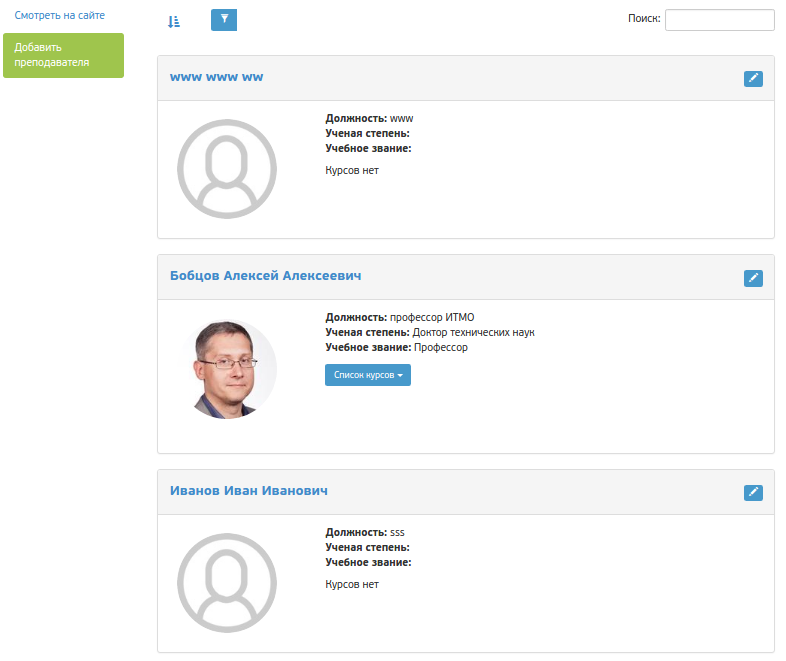
\includegraphics[width=1\linewidth]{list.png}}
	\caption{Внешний вид подраздела \quotes{Список преподавателей}}
	\label{instructor:list}
	\end{figure}
	
В центральной части страницы выводится непосредственно список преподавателей, каждый элемент которого "--- блок с краткой информацией о конкретном преподавателе. В левом углу верхней панели блока ФИО является ссылкой, ведущей в подраздел \quotes{Просмотр профиля преподавателя}, в правом углу "--- иконка редактирования, нажатие которой переводит в подраздел \quotes{Редактирование профиля преподавателя}. В основной части блока показаны:
\begin{itemize}
	\item фотография профиля, если она загружена или изображение по умолчанию, если отсутствует;
	\item должность преподавателя в вузе;
	\item ученая степень;
	\item учебное звание;
	\item список курсов. (показать/скрыть список курсов можно нажатием на кнопку \quotes{Список курсов} в блоке соответствующего преподавателя).
\end{itemize}

Вид блока с развернутым списком курсов приведён на рисунке~\ref{instructor:list_courses}.
	
	\begin{figure}[H]
	\center{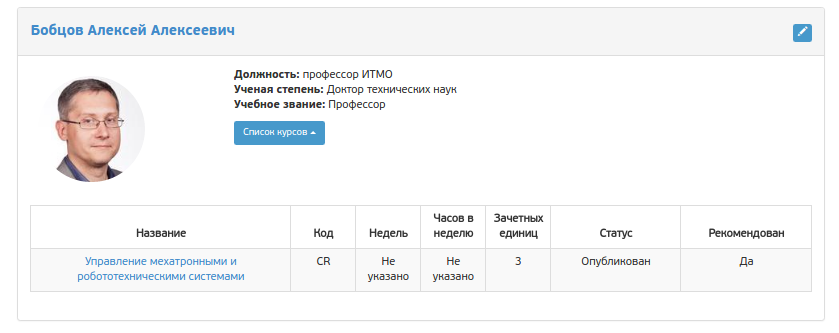
\includegraphics[width=1\linewidth]{list_courses.png}}
	\caption{Вид элемента списка преподавателей}
	\label{instructor:list_courses}
	\end{figure}

\subsubsection{Элементы управления}
На странице списка преподавателей присутствуют следующие элементы управления:
\begin{itemize}
	\item Кнопки \quotes{Смотреть на сайте} и \quotes{Добавить преподавателя}. Расположены на панели слева от списка преподавателей. По нажатию кнопки \quotes{Смотреть на сайте} происходит перенаправление на страницу университета на сайте, которая видна для пользователей. \\
	По нажатию кнопки \quotes{Добавить преподавателя} происходит перенаправление в соответствующий раздел.
	\item Иконка изменения порядка отображения преподавателей 	\vcenteredinclude[width=0.1\linewidth]{list_order.png}. 


По умолчанию список отсортирован в алфавитном порядке по ФИО в направлении А--Я, нажатие на иконку изменяет порядок на противоположный.
	\item Иконка вызова формы фильтрации \vcenteredinclude[width=0.1\linewidth]{list_filter_icon.png}.

 
По умолчанию в списке показаны все преподаватели вуза, однако, можно осуществить фильтрацию и вывести только тех, которые удовлетворяют параметрам, указным в форме фильтрации. По нажатию на иконку всплывает окно с формой фильтрации, в которой можно задать интересующие параметры (см. рис.~\ref{instructor:list_filter_form}). 

	\begin{figure}[H]
	\center{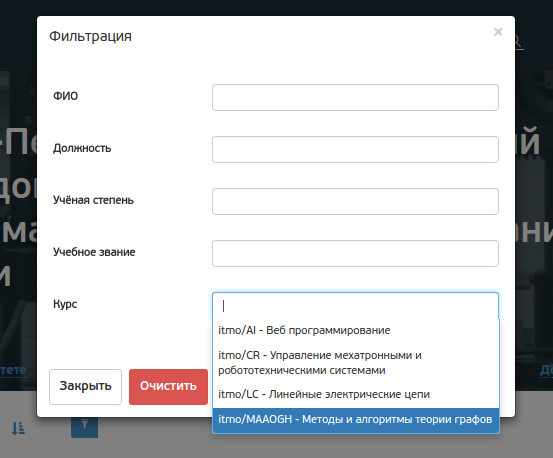
\includegraphics[width=1\linewidth]{list_filter_form.png}}
	\caption{Форма фильтрации}
	\label{instructor:list_filter_form}
	\end{figure}

Форма содержит следующие поля:
\begin{itemize}
	\item ФИО преподавателя (для поиска можно вводить любые части и комбинации фамилии, имени, отчества);
	\item должность;
	\item учёная степень;
	\item учебное звание;
	\item курс (принципы работы с полями такого типа описаны в подразделе ~\ref{widget:autocomplete_with_multiselect});
\end{itemize}	

Для того, чтобы применить фильтр необходимо нажать кнопку формы \quotes{Фильтровать}, после этого в списке останутся только преподаватели, удовлетворяющие введенным параметрам, а на верхней панели подраздела появится красная иконка \quotes{Отменить фильтр} \vcenteredinclude[width=0.2\linewidth]{list_filter_cancel.png}


Нажатие на эту кнопку отменяет применённый фильтр, в списке снова отображаются все преподаватели.
Пример результата фильтрации приведён на рисунке~\ref{instructor:list_filter_result}.

	\begin{figure}[H]
	\center{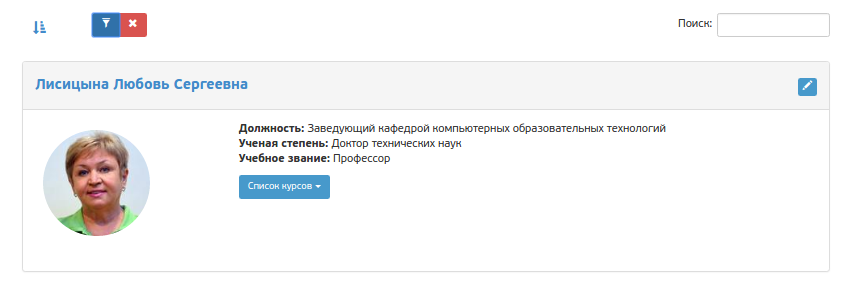
\includegraphics[width=1\linewidth]{list_filter_result.png}}
	\caption{Результат применения фильтра}
	\label{instructor:list_filter_result}
	\end{figure}
	
	\item Поле быстрого поиска расположено в правом углу верхней панели раздела, справа от метки \quotes{Поиск}. Поиск осуществляется по ФИО преподавателя, при заполнении поля выводятся только те преподаватели, чьи ФИО содержат введенную в поле строку (см. рис. ~\ref{instructor:list_search}).
	
	\begin{figure}[H]
	\center{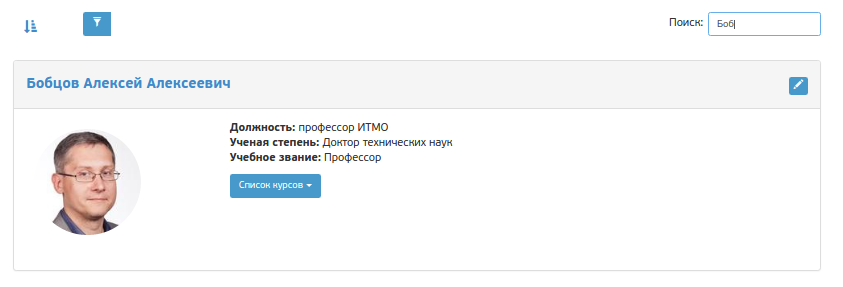
\includegraphics[width=1\linewidth]{list_search.png}}
	\caption{Применение быстрого поиска}
	\label{instructor:list_search}
	\end{figure}
	
	\item Элемент постраничной навигации \vcenteredinclude[width=0.3\linewidth]{list_pagination.png}         
 расположен внизу страницы раздела. На одной странице выводятся пять элементов списка, для перехода на следующую/предыдущую страницу используются стрелки вправо/влево.
	
\end{itemize}


\subsection{Просмотр профиля преподавателя}\label{instructor:detail_section}
По нажатию на ФИО интересующего преподавателя в списке преподавателей открывается относящийся к нему подраздел \quotes{Просмотр профиля преподавателя}, в котором доступны для просмотра все имеющиеся на текущий момент данные о преподавателе:
\begin{itemize}
	\item фото;
	\item ФИО;
	\item должность;
	\item ученая степень;
	\item учебное звание;
	\item образование;
	\item описание;
	\item профессиональный опыт;
	\item награды и достижения;
	\item внешние ресурсы;
	\item номер в списке преподавателей (на сайте преподаватели выводятся в порядке, соответствующем их номерам, по возрастанию номеров);
	\item опубликован "--- cтатус видимости преподавателя на сайте. (если значение статуса \quotes{Да} "--- преподаватель виден на сайте, иначе "--- скрыт);
	\item курсы (если на портале есть курсы, относящиеся к этому преподавателю, то на странице отображается таблица, содержащая информацию об этих курсах).
\end{itemize}
Внешний вид подраздела приведён на рисунке~\ref{instructor:detail}.

	\begin{figure}[H]
	\center{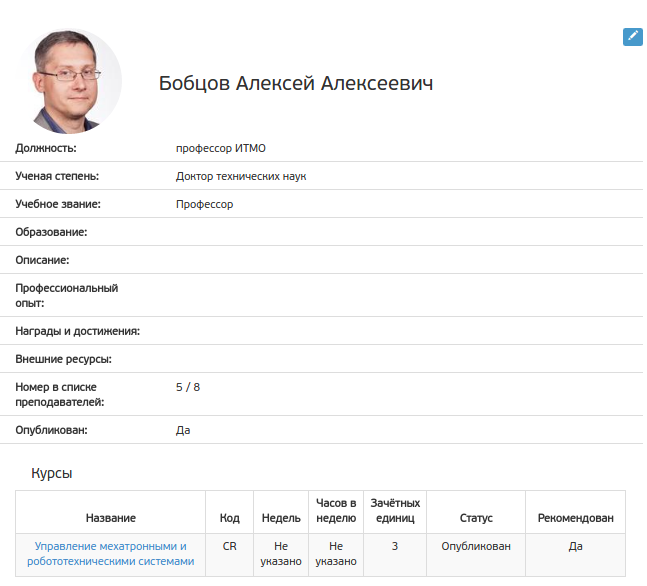
\includegraphics[width=1\linewidth]{detail.png}}
	\caption{Внешний вид подраздела \quotes{Просмотр профиля преподавателя}}
	\label{instructor:detail}
	\end{figure}
	
\subsection{Редактирование профиля преподавателя}\label{instructor:edit_section}
Перейти в этот подраздел можно, нажав иконку редактирования \vcenteredinclude[width=0.1\linewidth]{edit_icon.png} в блоке преподавателя в списке или в верхнем правом углу подраздела \quotes{Просмотр профиля преподавателя}.


В этом случае осуществляется переход к форме редактирования профиля преподавателя, в которой можно изменять поля, описанные в подразделе~\ref{instructor:detail_section} за исключением курсов, редактирование которых осуществляется в разделе \quotes{Курсы}. 

\subsubsection{Поля и ошибки}
	В форме представлено несколько типов полей:
	\begin{itemize}
		\item \textbf{Обязательные поля} отмечены символом \quotes{*}, если такое поле оставить не заполненным "--- появляется сообщение о необходимости его заполнения и блокируется кнопка сохранения изменений (см. рис.~\ref{instructor:edit_required}).
		
		\begin{figure}[H]
		\center{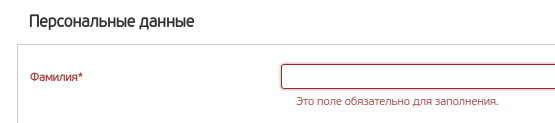
\includegraphics[width=1\linewidth]{edit_required.png}}
		\caption{Обработка заполнения обязательных полей}
		\label{instructor:edit_required}
		\end{figure}	
		
		\item \textbf{Поле \quotes{порядок преподавателей}} представляет собой список ФИО преподавателей, относящихся к тому же университету, что и тот, чей профиль редактируется. ФИО отображаются в том порядке, в котором они будут показаны на сайте, изменить порядок можно, перетащив стрелкой мыши выбранную строку на новую позицию. Строка с редактируемым преподавателем выделена границей и более темным фоном (см. рис.~\ref{instructor:edit_instructors}). Описание работы с виджетом изменения порядка см. в подразделе~\ref{widget:ordering}.
		
		\begin{figure}[H]
		\center{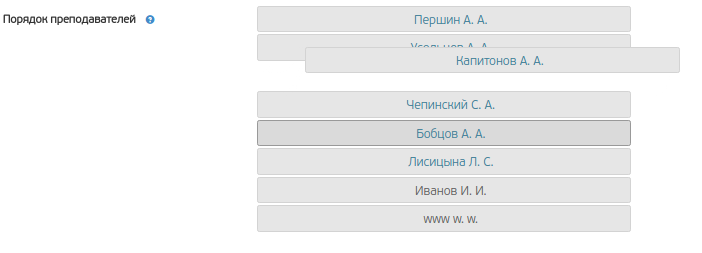
\includegraphics[width=1\linewidth]{edit_instructors.png}}
		\caption{Изменение порядка преподавателей}
		\label{instructor:edit_instructors}
		\end{figure}	
		
Видимость преподавателя на сайте настраивается путем переключения значения поля \quotes{Опубликован}. Неопубликованные преподаватели скрыты на сайте для пользователей. В форме в списке преподавателей показываются как скрытые, так и опубликованные преподаватели. В зависимости от статуса их ФИО имеют различный цвет, подробное описание можно получить, нажав на иконку \quotes{помощь} рядом с меткой поля (см. рис.~\ref{instructor:edit_instructors_legend}).
		
		\begin{figure}[H]
		\center{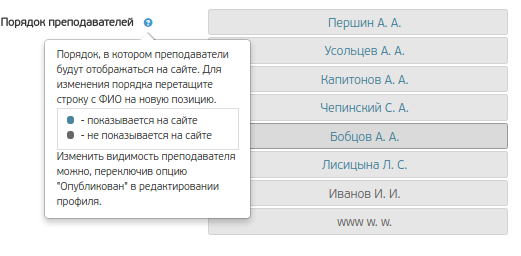
\includegraphics[width=1\linewidth]{edit_instructors_legend.png}}
		\caption{Справка о статусе преподавателей}
		\label{instructor:edit_instructors_legend}
		\end{figure}	
		
		\item \textbf{Файлы}. Форма редактирования позволяет загрузить фото профиля для отображения на страницах университета  и курсов преподавателя. Слева под меткой поля показано текущее загруженное изображение, если оно есть (см рис.~\ref{instructor:edit_logo}) или изображение по умолчанию, если ничего не загружено (см рис.~\ref{instructor:edit_icon_image}). Подробная информация о работе с файловыми полями приведена в разделе~\ref{widget:file_upload}.
		
		\begin{figure}[H]
		\center{
\includegraphics[width=1\linewidth]{edit_logo.png}}
		\caption{Файловое поле с загруженным изображением}
		\label{instructor:edit_logo}
		\end{figure}	
		
		\begin{figure}[H]
		\center{
\includegraphics[width=1\linewidth]{edit_icon_image.png}}
		\caption{Файловое поле с изображением по умолчанию}
		\label{instructor:edit_icon_image}
		\end{figure}
\end{itemize}

	\subsubsection{Элементы управления}

Управление внесенными изменениями осуществляется с помощью кнопок, расположенных внизу страницы (см. рис.~\ref{instructor:edit_buttons}).
		\begin{figure}[H]
		\center{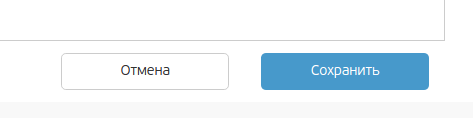
\includegraphics[width=1\linewidth]{edit_buttons.png}}
		\caption{Элементы управления подраздела \quotes{Редактирование профиля преподавателя}}
		\label{instructor:edit_buttons}
		\end{figure}	
		
При нажатии \quotes{сохранить} осуществляется попытка сохранения формы: если форма заполнена корректно, то внесенные изменения сохраняются, пользователь перенаправляется в раздел \quotes{Просмотр профиля преподавателя}, в противном случае "--- отображаются сообщения об ошибках, осуществляется прокрутка к месту первой ошибки. 


При нажатии кнопки \quotes{отмена} все изменения теряются, пользователь перенаправляется на предыдущую страницу.



\subsection{Создание преподавателя}
Перейти к созданию преподавателя можно, нажав на кнопку \quotes{Добавить преподавателя}, которая размещена на левой панели во всех подразделах раздела \quotes{Преподаватели}. В этом случае осуществляется переход к форме создания нового преподавателя, в которой возможно задать значения полей, описанных в разделе~\ref{instructor:detail_section}. Содержание, возможные действия и реакции в этом разделе аналогичны описанным в разделе \quotes{Редактирование профиля преподавателя}~\ref{instructor:edit_section} за исключением вида поля \quotes{Порядок преподавателей}.



\textbf{Поле \quotes{Порядок преподавателей}} представляет собой список ФИО преподавателей, относящихся к университету, в кабинете которого находится пользователь. Строка, описывающая нового преподавателя, вместо ФИО содержит текст \quotes{Добавить на эту позицию}, кроме того, она выделена среди остальных более темным цветом фона и темной границей.


Строки отображаются в порядке, в котором преподаватели будут показаны на сайте, новый преподаватель по умолчанию помещается на последнюю позицию, изменить порядок можно, перетащив  при помощи мыши выбранную строку на новую позицию. (см. рис.~\ref{instructor:create_instructors}).
		
		\begin{figure}[H]
		\center{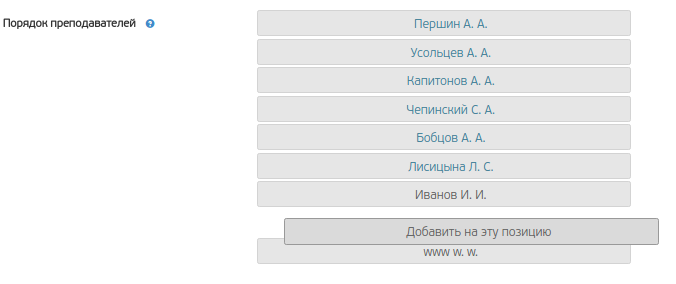
\includegraphics[width=1\linewidth]{create_instructors.png}}
		\caption{Изменение порядка преподавателей}
		\label{instructor:create_instructors}
		\end{figure}	
		
Видимость преподавателя на сайте настраивается путем переключения значения поля \quotes{Опубликован}. Неопубликованные преподаватели скрыты на сайте для пользователей. В форме в списке преподавателей показываются как скрытые, так и опубликованные преподаватели, в зависимости от статуса их ФИО имеют различный цвет. Подробное описание можно получить, нажав на иконку \quotes{помощь} рядом с меткой поля (см. рис.~\ref{instructor:create_instructors_legend}).
		
		\begin{figure}[H]
		\center{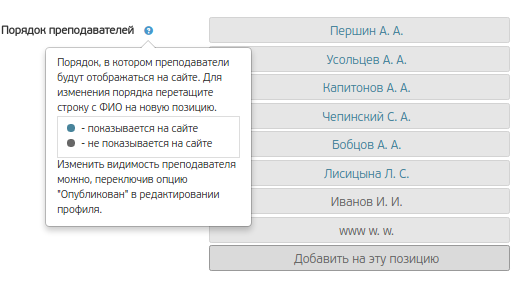
\includegraphics[width=1\linewidth]{create_instructors_legend.png}}
		\caption{Справка о статусе преподавателей}
		\label{instructor:create_instructors_legend}
		\end{figure}	
